\documentclass[12pt]{ut-thesis}

% ----------------------------------------------------------------------------------------------------------------------------------------
% USEPACKAGE DECLARATIONS
% ----------------------------------------------------------------------------------------------------------------------------------------

%\includeonly{./sections/reionization}

\usepackage{amsmath}
\usepackage{amssymb}
\usepackage{aas_macros}
\usepackage{natbib}
\usepackage{html}
\usepackage{graphicx}
\usepackage{rotating}
\usepackage{tabularx}
\usepackage{pdflscape}
\usepackage{afterpage}
\usepackage{capt-of}
%\usepackage[figuresleft]{rotating}

% ----------------------------------------------------------------------------------------------------------------------------------------
% AUTHOR INFORMATION
% ----------------------------------------------------------------------------------------------------------------------------------------

\degree{Doctor of Philosophy}
\department{Astronomy and Astrophysics}
\gradyear{2016}
\author{Liam Dean Connor}
\title{Long wavelength astrophysics}

% ----------------------------------------------------------------------------------------------------------------------------------------
% COMMANDS AND DEFINITIONS
% ----------------------------------------------------------------------------------------------------------------------------------------

% Put here all other formatting commands that belong in the preamble. In particular, you should put all of 
% your \newcommand's, \newenvironment's, \newtheorem's, etc. (in other words, all the global definitions 
% that you will need throughout your thesis) in a separate file and use "\input{filename}" to input it here.
\input{commands}

% Table of contentds depth (0 = chapter, 1 = section, 2 = subsection, 3 = subsubsection, etc.)
\setcounter{tocdepth}{2}

% Make each page fill up the entire page.
\flushbottom

% ==============================================================================
% PRELIMINARY CONTENT
% ==============================================================================

\begin{document}

% This sets the page style and numbering for preliminary sections.
\begin{preliminary}

% This generates the title page from the information given above.
\maketitle

% There should be NOTHING between the title page and abstract.  However, if your document 
% is two-sided and you want the abstract _not_ to appear on the back of the title page, then uncomment 
% the following line.
% \cleardoublepage

% ----------------------------------------------------------------------------------------------------------------------------------------
% ABSTRACT
% ----------------------------------------------------------------------------------------------------------------------------------------

\begin{abstract} % At most 350 words for Ph.D.

\end{abstract}

% Anything placed between the abstract and table of contents will appear on a separate page since the 
% abstract ends with \newpage and the table of contents starts with \clearpage.  Use \cleardoublepage
% for anything that you want to appear on a right-hand page.

% ----------------------------------------------------------------------------------------------------------------------------------------
% DEDICATION
% ----------------------------------------------------------------------------------------------------------------------------------------

%\begin{dedication}
\vspace*{\fill}
\begin{center}
{\em To Pop and my infinitely supportive parents}
\end{center}
\vfill
%\end{dedication}

\newpage % Force separate pages for dedication and acknowledgements


% ----------------------------------------------------------------------------------------------------------------------------------------
% ACKNOWLEDGEMENTS
% ----------------------------------------------------------------------------------------------------------------------------------------

\begin{acknowledgements}

\end{acknowledgements}

% ----------------------------------------------------------------------------------------------------------------------------------------
% TABLE OF CONTENTS
% ----------------------------------------------------------------------------------------------------------------------------------------

\tableofcontents

% ----------------------------------------------------------------------------------------------------------------------------------------
% LIST OF TABLES
% ----------------------------------------------------------------------------------------------------------------------------------------

\listoftables

% ----------------------------------------------------------------------------------------------------------------------------------------
% LIST OF FIGURES
% ----------------------------------------------------------------------------------------------------------------------------------------

%\listoffigures

\end{preliminary}

% ==============================================================================
% CHAPTERS
% ==============================================================================

%%%%%%%%%%%%%%%%%%%%%%%%%%%%%%%%%%%%%%%%%%%%%%%%%%%%%%%%%%%%%%%%%%%%%%%%
%%  Put your Chapters here; the easiest way to do this is to keep     %%
%%  each chapter in a separate file and `\include' all the files.     %%
%%  Each chapter file should start with "\chapter{ChapterName}".      %%
%%  Note that using `\include' instead of `\input' will make each     %%
%%  chapter start on a new page, and allow you to format only parts   %%
%%  of your thesis at a time by using `\includeonly'.                 %%
%%%%%%%%%%%%%%%%%%%%%%%%%%%%%%%%%%%%%%%%%%%%%%%%%%%%%%%%%%%%%%%%%%%%%%%%

%\include{./sections/introduction}
\chapter{Beamforming}
\label{chapter:beamforming}
\chaptermark{Relative velocity reconstruction}



% ================================================================================
% CHAPTER OVERVIEW
% ================================================================================

\section{Chapter Overview}

Beamforming
% ================================================================================
% INTRODUCTION
% ================================================================================

\section{Introduction}


  
% ================================================================================
% THEORY AND IMPLEMENTATION
% ================================================================================
  
\section{Theory and Implementation}
\label{sec:theory}

Beamforming is a signal processing technique that allows for 
spatial filtering, and has greatly benefited a diverse set of fields 
from radar and wireless communications to radio astronomy. % Insert history

By coherently combining the voltages of a multi-element array, 
sensitivity can be allocated to small regions of the sky and 
the array's effective forward gain can be increased. The signal 
from each antenna, $x_n$, is multiplied by a complex weight, whose 
phases, $\phi_n$, are chosen to destructively interfere the radio waves 
in all directions but the desired pointing. The signals 
from all antennas are then combined to give the formed beam 
voltage stream, $X_{\rm BF}$.

\begin{equation}
\label{eq-bf_sum}
X_{\rm BF} = \sum_{n=1}^N a_n e^{i\phi_n} x_n
\end{equation}

\noindent Here $a_n$ are real numbers that can be used to as 
amplitude weightings for the antennas. If we define a more 
general complex weighting, $w_n \equiv a_n e^{i\phi}$, and 
switch to vector notation, Eq.~\ref{eq-bf_sum} becomes,



\begin{align}
\rm{sin}(alt) = \rm{sin}(\delta)\, \rm{sin}(lat) + cos(\delta)\, cos(lat)\, cos(\rm HA)\\
\rm{cos}(az) = \frac{\rm{sin}\delta - \rm{sin}(alt) \,
\rm{sin}(lat)}{\rm{cos}(alt)\, \rm{cos}(lat)}
\end{align}

\subsection{Neutrino $N$-body Particles in \cpm{}}
\label{}

We simulate a single neutrino species as an $N$-body particle. Initial neutrino positions are generated separately from CDM using the same Gaussian noise map. We use neutrino density transfer functions, $\tdel$, computed via \camb{} \citep{lewis/etal:2000} for a universe with one massive and two massless neutrinos. The initial neutrino velocity is composed of two parts: a linear component (analogous to the Zel'dovich velocity) plus a random thermal component.  For the linear component, we first compute the linear neutrino velocity transfer function, $\tvel$, via the continuity equation under the assumption that initial conditions are adiabatic and velocities are linear (e.g. $\delta(k,z) = \tdel(k,z) \delta_i(k)$ and $\vec{v}(\vec{k},z) = \tvel(k,z) \delta_i(k) \hat{k}$ for an initial perturbation $\delta_i(k)$):
\bq
\dot{\delta} + \frac{1}{a}\vec{\nabla}\cdot\vec{v} = 0 \rightarrow \tvel = - i \frac{H}{k} \frac{\tdel(z+\delta z) - \tdel(z-\delta z)}{2 \delta z},
\label{eq:veltransfer}
\eq
where we convert time derivatives to redshift derivatives and evaluate numerically using a spacing $\delta z = 0.1$. We have checked that the transfer functions computed via equation \ref{eq:veltransfer} are in good agreement with those produced by the {\small CLASS} code \citep{blas/etal:2011} in Newtonian gauge\footnote{The {\small CAMB} density transfer functions are in the synchronous gauge whereas the velocity transfer function we desire are in the longitudinal Newtonian gauge.  However, the gauge transformation terms are proportional to the time derivatives of the Newtonian potentials which we already ignore in the continuity equation.}.  
  
From this velocity transfer function, we compute a velocity potential, $\phi_v(k)$, such that $\vec{v}(k) = i \vec{k} \phi_v(k) = (\tvel/\tdel)\delta \hat{k}$. When combined with equation \ref{eq:veltransfer} this yields:
\bq
\phi_v(k) = - \frac{H}{k} \frac{\tdel(z+\delta z) - \tdel(z-\delta z)}{2 \delta z} \frac{\delta}{\tdel}.
\label{eq:velpotential}
\eq
This potential is then Fourier transformed and a two-sided finite difference is taken to obtain the linear velocity.  Using a real-space gradient reduces the number of Fourier transforms to be computed and is consistent with our calculation of the displacement field.  

The random component of the velocity is computed via the
cumulative distribution function, ${\rm CDF}[v,\beta]$, which
follows from the relativistic Fermi-Dirac distribution,
${\rm PDF}[v,\beta]$, for neutrinos:
\bqa
{\rm PDF}[v,\beta] &= & \frac{1}{N}\left(\frac{m_\nu}{kT}\right)^3\frac{v^2}{e^{m_\nu v/kT}+1} = \frac{\beta^3}{N}\frac{v^2}{e^{v\beta}+1} \nonumber \\
{\rm CDF}[v, \beta] &=& \int_0^v {\rm PDF}[u,\beta] du \nonumber   \\
                              &=&\frac{1}{N} \int_0^{w=\beta v} \frac{w^2}{e^w+1}dw \nonumber \\
                              &=&{\rm CDF}[\beta v,1]
\label{eq:fermicdf}
\eqa
where $m_\nu$ and $T$ are neutrino mass and temperature, respectively, $\beta \equiv m_\nu/kT$ and $N = \int_0^\infty w^2/(e^w+1) dw \simeq 1.803$ is a normalization constant.  Our numerical evaluation of the $\rm CDF$ gives a maximum particle speed of $0.013 \left(0.2\:\ev/m_\nu\right) (1+z_i)c$ for a given starting redshift $z_i$.  Neutrinos in the mass regime we are interested in are relativistic at the redshift for which CDM initial conditions are generated ($z_c = 100$):
\bq
\langle v \rangle = \frac{\int_0^\infty v{\rm PDF}[v,\beta] dv}{\int_0^\infty {\rm PDF}[v,\beta] dv} \approx 800 \left(\frac{0.2\ \ev}{m_\nu}\right) (1+z)\ \kms.
\eq
This thermal motion would dominate the time step constraining the maximum distance a particle may travel, making the simulation impractically slow.  To circumvent this issue we evolve the CDM in isolation to a lower redshift, $z_\nu \sim 10$, at which point neutrinos are added and the two components evolve together.
  
During their subsequent evolution, CDM and neutrino particles are treated identically except for their masses, which are weighted by their energy fractions as well as number ratio:
\bq
m_i = \frac{\Omega_i}{\Omega_m}\frac{N_g}{N_i},
\label{eq:pmass}
\eq
where $\Omega_i$ is the energy fraction of species $i$, $\Omega_m$ is the total matter energy fraction, $N_g$ is the number of cells in the simulation grid, and $N_i$ is the number of particles of species $i$.  These masses are used when adding particles to the grid for the computation of the long-range gravitational force as well as the short-range pairwise force.  The particle type is distinguished within the code using 1 byte particle identification tags.  

\subsection{Density and Velocity Fields}
\label{ssec:velocity}

We compute CDM, neutrino, and halo density fields using a standard cloud-in-cell interpolation method for both CDM and neutrinos. Computing velocity fields from particle-based simulations has only recently been studied in depth. This may be related to the ambiguity associated with defining a velocity field from a sample of point particles. Unlike quantities such as mass or momentum, the velocity of a particle cannot be simply added to a grid. The most obvious method for generating a velocity field is to divide a gridded momentum field by its corresponding density field. However, within void regions it is possible that empty cells exist for which no well-defined velocity can be assigned. Alternatively, one may define the velocity at a given grid cell to be the average velocity of the $N_{\rm near}$ nearest particles about this point.  The application of the nearest particle method was studied by \citet{zhang/etal:2015} and \citet{zheng/etal:2015} where it was found that the velocity power is suppressed for low particle number densities, $n<1\ (\mpch)^{-3}$, due to the sampling procedure.  In our simulations we use high number densities, $n_{\rm dm} \sim 10\ (\mpch)^{-3}$, and therefore do not expect this effect to be significant.  More advanced methods for computing velocity fields exist such as phase-space interpolation discussed in \citet{pueblas/scoccimarro:2009} and more recently in \citet{hahn/etal:2014}.  The neutrino velocity distribution has been studied by \citet{villaescusa-navarro/etal:2013}.
  
In what follows we compute the velocity fields of CDM and neutrinos in different ways.  For CDM, we adopt the nearest particle method and take the $N_{\rm near} = 1$ nearest particle about the centre of each cell using the same grid resolution as neutrinos.  We have found that the nearest particle method can also be used for neutrinos albeit with a much larger $N_{\rm near} = 64$ to smooth the field on small scales. However, searching over this many particles is a computationally expensive task.  For neutrinos we therefore employ the approach of dividing their momentum field by their density field on grids coarsened so that there is always at least one neutrino per cell. This is possible since neutrinos are rather homogeneously distributed and form voids to a lesser extent than CDM.

We treat the velocity fields obtained from the nearest particle and momentum methods as faithful tracers of the actual field. However, these fields are not comparable to observational data since neither CDM nor neutrino velocities can be directly measured.  For this purpose we reconstruct velocity fields from density fields using linear theory:
\bq
\vec{v} = \frac{\tvel}{\tdel}\frac{\vec{k}}{k}\delta,
\label{eq:vrec}
\eq
where we use CDM and halo density fields separately for $\delta$ (although with the same $\tdel$).  In what follows we treat halos as point particles of unit mass in order to represent the information available through galaxy surveys.  
  
Poisson noise is a severe hindrance in computing neutrino statistics as the large thermal velocity causes neutrino particles to be more homogeneously distributed.  For density spectra it is possible to subtract out the flat Poisson noise spectrum but this is not possible for velocity fields.  Instead, we use a method that exploits the fact that Poisson noise arises from particles being randomly distributed.  The procedure for either density or velocity fields is:
\begin{enumerate}
\item Randomly divide the particles into two groups.
\item Interpolate particles of each group into a field (density or velocity).
\item Compute the cross spectrum between groups as an estimate of the auto spectrum.
\end{enumerate}
This procedure ensures that Poisson noise is highly suppressed as the noise between the two groups is uncorrelated due to the random assignment to groups.  We use this method for density and velocity auto-spectra for both CDM and neutrinos; we do not use it for CDM-neutrino cross spectra where it is redundant (there are already two groups of particles).  
  
The accuracy of the reconstructed field is measured using a correlation coefficient:
\bq
r_{ij}(k) = \frac{\Delta^2_{ij}(k)} { \sqrt{\Delta^2_{ii}(k)\Delta^2_{jj}(k)} }
\label{eq:rij} 
\eq
where $\Delta^2_{ij}$ is the cross power spectrum between species $i=c,h,\nu \textrm{ or rel}$ using reconstruction method $\mbox{sim}, \mbox{Rec DM}, \mbox{Rec HA}$ (nearest particle/momentum, equation \ref{eq:vrec} with CDM and equation \ref{eq:vrec} with haloes respectively) and species $j$ (with potentially a different reconstruction method).  We also define the integrated correlation coefficient as:
\bq
r_{ij} = \frac{\int \Delta^2_{ij} \frac{dk}{k}}{\sqrt{\int \Delta^2_{ii} \frac{dk}{k}} \sqrt{\int \Delta^2_{jj} \frac{dk}{k}}}
\label{eq:intrij}
\eq
which no longer depends on wavenumber.
  
% ================================================================================
% RESULTS
% ================================================================================  
  
\section{Results}
\label{sec:nu-results}

In this section we present the results for a suite of four simulations of CDM and neutrinos.  We simulate neutrinos of mass $m_\nu = 0.4, 0.2, 0.1$ and $0.05\:\ev{}$.  Each simulation contains $N_c = 1536^3$ CDM particles and $N_\nu = 3072^3$ neutrino particles within a periodic box of side length $L = 500\ \mpch$. In each case CDM is started from an initial redshift $z_c = 100$ and gravitational forces are softened below the scale $r_{\rm soft} = 24$ kpc/$h$.  Neutrinos are added in at redshift $10$ for all species except $0.05\:\ev{}$ which we add at redshift $5$.  We assume a base cosmology compatible with Planck results: $\Omega_b = 0.05$, $\Omega_c = 0.27$, $\sigma_8 = 0.83$, $n_s = 0.96$, $h = 0.67$, and compute
\bq
\Omega_{\nu} = \frac{m_\nu}{93.14\ h^2}
\label{eq:omnu}
\eq
as in \citet{mangano/etal:2015}. We hold $\Omega_b$ and $\Omega_c$ fixed in each simulation and maintain a flat universe by adjusting $\Omega_\Lambda = 1 - \Omega_m = 1 - \Omega_b - \Omega_c - \Omega_\nu$. In what follows we mainly investigate a fiducial simulation with $m_\nu = 0.2$ eV.  We label our simulations based on neutrino mass with S05, S1, S2, and S4 denoting the simulations with $m_\nu = 0.05, 0.1, 0.2$, and $0.4\:\ev{}$ respectively.  

Halo catalogues are generated for each simulation at $z = 0$ using a spherical overdensity algorithm that considers all halos with at least 100 CDM particles. This corresponds to a minimum halo mass of $3 \times 10^{11}\ M_\odot/h$. Recall, however, that we assign each halo unit mass when constructing halo density fields in order to emulate the information available in galaxy surveys. In what follows, density and velocity fields for CDM, neutrinos, and halos are computed on uniform rectilinear grids containing $1536^3$ mesh cells.  
    
\subsection{Density}
\label{ssec:density}

% -------------------------------------------- FIGURE 1 --------------------------------------------
\begin{figure}
\begin{center}
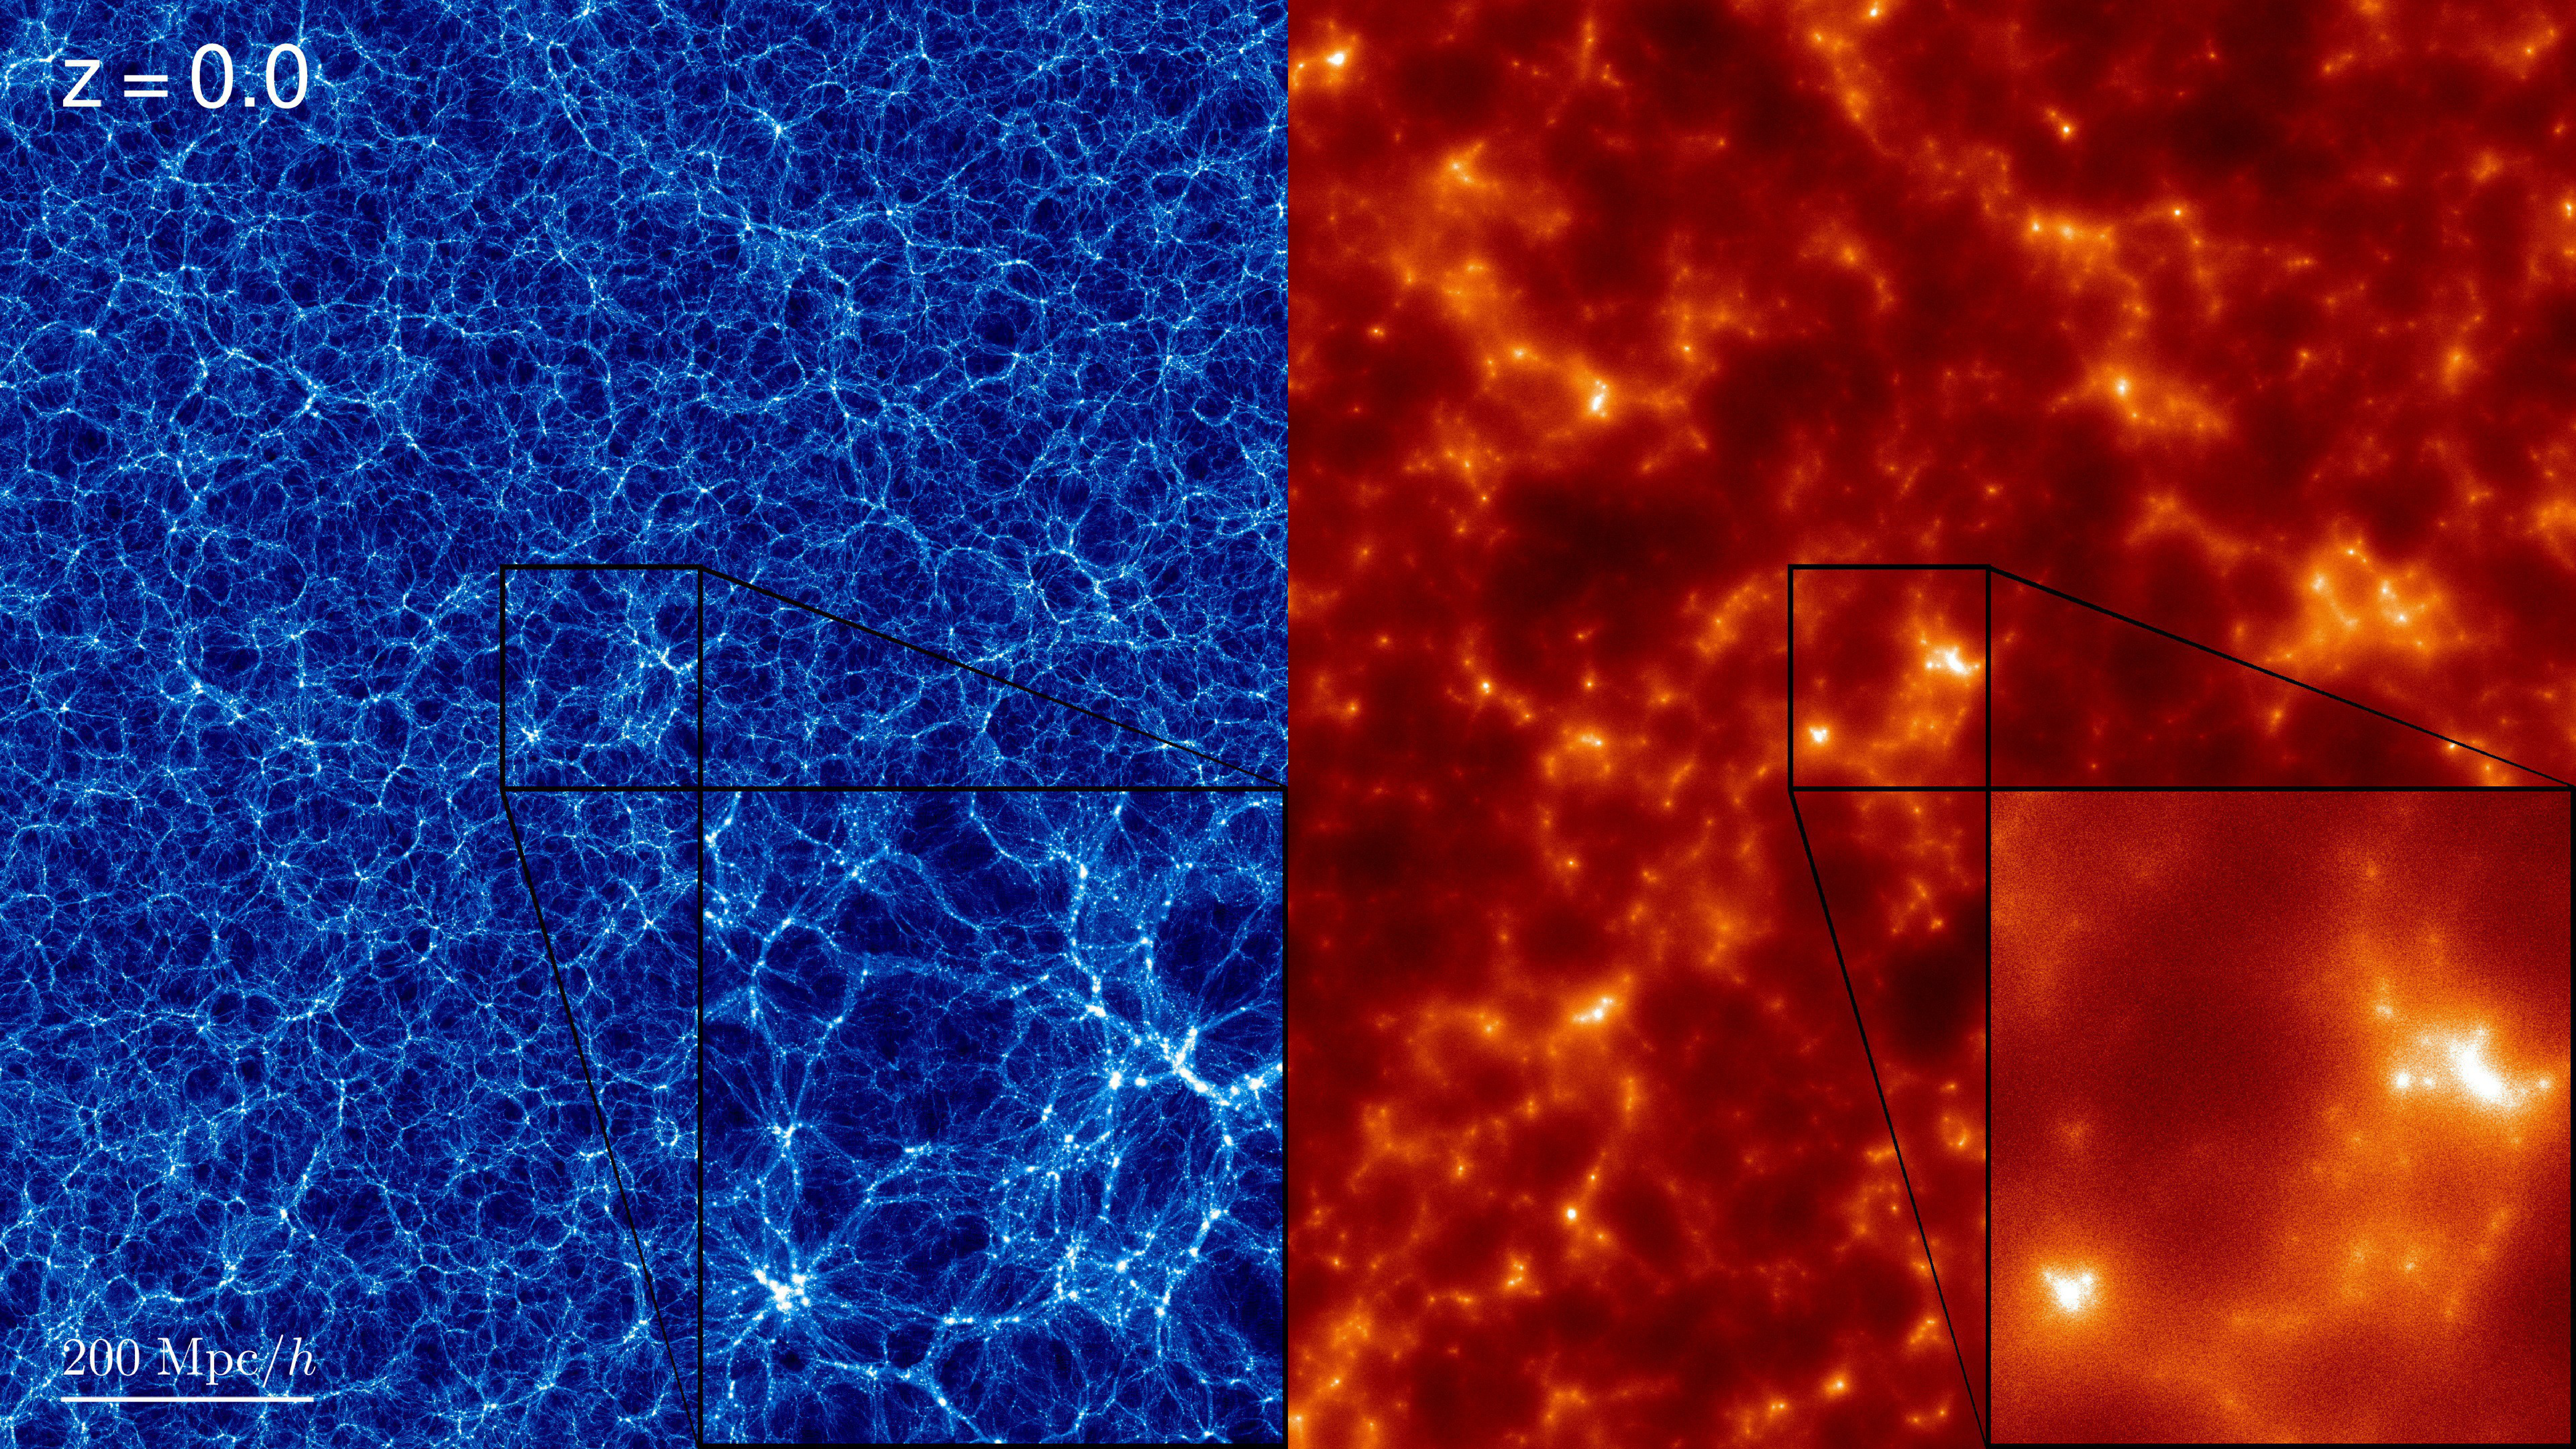
\includegraphics[width=0.85\textwidth]{./figures/neutrinos/fig1.pdf} \vspace{-0.1cm}
\caption[Cold dark matter, neutrino, and halo density slices]
{Density slices of equal width $500\ \mpch{}$ and
thickness $1.3\ \mpch{}$ from various simulations at
$z = 0$.  The top row shows cold dark matter (left) and halo
(right) density slices from the 0.2\ \ev{} neutrino
simulation. The middle row compares neutrino density slices
from the 0.05 (left) and 0.1 (right)\ \ev{} simulations
while the bottom row shows the 0.2 (left) and 0.4 (right)\
\ev{} simulations.  It is easy to see by eye that the cold dark
matter and neutrino density fields are highly correlated and
that heavier neutrinos cluster more than lighter ones.}
\vspace{-0.5cm}
\label{fig:denslice}
\end{center}
\end{figure}
% -------------------------------------------- FIGURE 1 --------------------------------------------

Figure \ref{fig:denslice} compares slices of the CDM and halo density fields at $z = 0$ from simulation S2 to the neutrino density fields from simulations S05, S1, S2, and S4.  It is easy to see that the neutrino density fields are correlated with the CDM density field albeit with much less clumping in the former than the latter as evidenced by their respective colour bars. In addition, we see that higher mass neutrinos tend to clump more than lower mass neutrinos as they are more influenced by the underlying CDM distribution due to their lower thermal velocities.

% -------------------------------------------- FIGURE 2 --------------------------------------------
\begin{figure}[!t]
\begin{center}
\includegraphics[width=\smwidth]{./figures/neutrinos/fig2.pdf} \vspace{-0.1cm}
\caption[Cold dark matter, neutrino, and halo density power spectra]
{The dimensionless matter power spectra at $z = 0$ for
cold dark matter (solid black line), halos (solid blue line)
and neutrinos (solid red line) from S2. Shot noise has been
removed by computing the cross-spectrum between two randomly
chosen groups for each species.  Also plotted are the linear
and nonlinear cold dark matter (dotted black and dashed
black lines) and neutrino (dotted red and dashed red lines)
power spectra. Note that there is a small numerical artifact
in the linear neutrino transfer function just above
$k = 1\:\hmpc$ that should be ignored.}
\vspace{-0.2cm}
\label{fig:denpow}
\end{center}
\end{figure}
% -------------------------------------------- FIGURE 2 --------------------------------------------

% -------------------------------------------- FIGURE 3 --------------------------------------------
\begin{figure}[!b]
\begin{center}
\includegraphics[width=\smwidth]{./figures/neutrinos/fig3.pdf} \vspace{-0.1cm}
\caption[Cold dark matter-neutrino cross correlation coefficient]
{The cold dark matter-neutrino cross correlation
coefficient at $z = 0$ from S2. As expected, neutrinos are
highly correlated with cold dark matter over a large range
of scales.}
\label{fig:dencorr}
\end{center}
\end{figure}
% -------------------------------------------- FIGURE 3 --------------------------------------------

Figure \ref{fig:denpow} shows the dimensionless power spectra for CDM, halos, and neutrinos at $z = 0$ from S2.  Also plotted are theoretical predictions for CDM and neutrinos, which are computed via
\bq
\Delta^2_i(k) = \frac{k^3}{2\pi^2}  P_m\left(\frac{T_i}{T_m}\right)^2,
\label{eq:PNL}
\eq    
where $T_i$ is the linear transfer function for species $i$, $T_m$ is the total matter linear transfer function, and $P_m$ is either the linear (computed from \camb{}) or the nonlinear [computed from \hfit{} \citep{smith/etal:2013}] total matter power spectrum. We first note that the group cross-correlation method we employ effectively removes the shot noise allowing us to understand statistical properties even of the noisy neutrino density field.  We find that the CDM power spectrum agrees well with the nonlinear prediction up to large $k$.  The neutrino power spectrum, on the other hand, is significantly enhanced on small scales compared to the theoretical curve demonstrating that the linear response of equation \ref{eq:PNL} fails to capture neutrino dynamics on small scales.  This trend was previously observed by Ali-Ha{\"i}moud (private communication) and modelled in \citet{massara/etal:2014}.

Despite their enhanced power on small scales, neutrinos remain highly correlated with the CDM density field, as was qualitatively discussed with Figure \ref{fig:denpow}.  More quantitatively, Figure \ref{fig:dencorr} shows the $z = 0$ cross-correlation coefficient between CDM and neutrinos from S2 as a function of wavenumber. We find that neutrinos exhibit $r_{c\nu} \gtrsim 0.9$ correlation with CDM on all scales $k < 1\ \hmpc$ and achieve $r_{c\nu} \sim 0.85$ down to the smallest scales resolved in the simulation.

The halo power spectrum is also plotted in Figure \ref{fig:denpow}. As expected, the halo power follows the general shape of the CDM power spectrum, but with a reduced amplitude, or bias.  We define the bias as:
\bq
b \equiv \sqrt{\frac{P_{hh}}{P_{cc}}},
\label{eq:bias}
\eq
and plot it as a function of $k$ in Figure \ref{fig:denbias}. Defining the bias with respect to the CDM power spectrum instead of the total matter spectrum (e.g. including neutrinos) was shown to be less scale dependent in \citet{castorina/etal:2014}. The bias is roughly constant on large scales with $b \sim 0.8$ and falls off on small scales as the halo density field does not include contributions from the ``one-halo'' term describing the internal mass profile of halos \citep{scherrer/bertschinger:1991}. Hence, halo power is suppressed on scales comparable to the typical virial radii of halos which occurs at $k \sim 0.2\ h/{\rm Mpc}$ for the largest halos in the box.

% -------------------------------------------- FIGURE 4 --------------------------------------------
\begin{figure}[!t]
\begin{center}
\includegraphics[width=\smwidth]{./figures/neutrinos/fig4.pdf} \vspace{-0.1cm}
\caption[Halo bias scale dependence]
{The halo bias parameter measured from S2 at $z = 0$.
On scales $k \lesssim 0.2\ h/{\rm Mpc}$ the bias is roughly
constant with $b \sim 0.8$. The bias falls off on smaller
scales as power is suppressed within the typical virial
radii of halos.}
\vspace{-0.2cm}
\label{fig:denbias}
\end{center}
\end{figure}
% -------------------------------------------- FIGURE 4 --------------------------------------------

\subsection{Velocity}

Figure \ref{fig:velslice} compares slices of CDM, neutrino, and CDM-neutrino relative velocity computed from the simulation particles as well as reconstructed from the CDM and halo density fields using equation (\ref{eq:vrec}). We observe a similar trend as the density fields with CDM and neutrinos highly correlated in velocity. In addition, we see that the velocity fields reconstructed from only knowledge of either the CDM or halo density field qualitatively agree with the large-scale structure of the velocity fields obtained within the simulation.

% -------------------------------------------- FIGURE 5 --------------------------------------------
\begin{figure}
\begin{center}
\includegraphics[width=0.99\textwidth]{./figures/neutrinos/fig5.pdf} \vspace{-0.1cm}
\caption[Slices of simulated and reconstructed velocity fields]
{Slices of equal width $500\ \mpch{}$ and thickness
$1.3\ \mpch{}$ showing the $z = 0$ velocity component
perpendicular to the page for cold dark matter (top row),
neutrinos (middle row), and the relative velocity between
cold dark matter and neutrinos (bottom row). Columns show
the velocity fields from the simulation particles (left
column), reconstructed from the cold dark matter density
field (middle column), and reconstructed from the halo
density field (right column). We see that both of the
reconstruction methods agree well with the large-scale
structure of the simulation velocity fields.}
\vspace{-0.5cm}
\label{fig:velslice}
\end{center}
\end{figure}
% -------------------------------------------- FIGURE 5 --------------------------------------------

Figure \ref{fig:velpow} compares the simulated CDM and neutrino velocity power spectra to the CDM and halo reconstructed fields. Note that for the latter we take $\delta = \delta_h/b$ in equation (\ref{eq:vrec}) to account for the halo bias. We use a value of $b = 0.80$ consistent with the large-scale bias found in Figure \ref{fig:denbias}.  We compute theoretical predictions for the velocity power using equation (\ref{eq:PNL}) with $T_i$ being a velocity transfer function.  We note that the groups method has also effectively removed shot noise from the velocity power just as for the density.
 
% -------------------------------------------- FIGURE 6 --------------------------------------------
\begin{figure}[!t]
\begin{center}
\includegraphics[width=\smwidth]{./figures/neutrinos/fig6.pdf} \vspace{-0.1cm}
\caption[Cold dark matter and neutrino velocity power spectra]
{Velocity power spectra at $z = 0$ from S2 for cold
dark matter (top) and neutrinos (bottom) normalized to the
linear theory result obtained from equation (\ref{eq:PNL}).  In
each panel, the dotted black line shows the nonlinear
expectation of equation (\ref{eq:PNL}), the solid black line shows
the simulation result, and the dashed blue line (dot-dashed
red line) shows the velocity field reconstructed from
equation (\ref{eq:vrec}) using the cold dark matter (halo) density field.}
\vspace{-0.2cm}
\label{fig:velpow}
\end{center}
\end{figure}
% -------------------------------------------- FIGURE 6 --------------------------------------------
 
Figure \ref{fig:velpow} demonstrates that the simulated CDM velocity field is suppressed on scales $0.2 \lesssim k \lesssim 4.0 \:\hmpc{}$ compared to the linear and nonlinear expectations. This suppression was also seen in \citet{pueblas/scoccimarro:2009,hahn/etal:2014} and may be due to the thermalization of CDM within collapsed objects.  The velocity field reconstructed from CDM agrees well with the nonlinear expectation of equation (\ref{eq:PNL}). This is simply a reflection of the agreement between the CDM density field and \hfit{} shown in Figure \ref{fig:denpow}. If we used the full bias curve, $b(k)$, instead of a constant then the halo reconstruction method works equally well.  Neutrinos, on the other hand, have a velocity power spectrum that agrees well with the nonlinear expectation on scales $k\lesssim 0.15 \:\hmpc$.  However, we find that they are underpredicted by linear theory on small scales.  It is unclear why neutrinos behave in an opposite manner from CDM.

The efficacy of reconstructing velocities using equation (\ref{eq:vrec}) relies on the linearity of the velocity field. To test this we decompose velocity into divergence and curl components. We have performed this computation using both real-space finite differencing of the velocity field as well as Fourier space decomposition:
\bqa
\vec{v}_k &= \hat{k}(\hat{k}\cdot\vec{v}_k) + \hat{k}\times(\hat{k}\times\vec{v}_k) \nonumber \\
                &=\hat{k}D +\vec{C},
\label{eqn:divcurl}
\eqa 
where $D$ is the divergence field and $\vec{C} = \vec{v}_k - \hat{k}D$ is the curl field. Both the real-space and Fourier-space methods produce equivalent results. In linear theory, the velocity is parallel to $\hat{k}$ and therefore has no curl. Hence, the presence of a curl component of the velocity field allows us to measure its degree of nonlinearity.
 
% -------------------------------------------- FIGURE 7 --------------------------------------------
\begin{figure}[!t]
\begin{center}
\includegraphics[width=\smwidth]{./figures/neutrinos/fig7.pdf} \vspace{-0.1cm}
\caption[Divergence and curl components of the cold dark matter and neutrino velocity power]
{Relative fraction of the divergence (solid black
line) and curl (dotted black line) components of the cold dark
matter (top) and neutrino (bottom) velocity power at $z = 0$
from S2. In each case, the curl component is negligible on
scales $k \lesssim 1\ \hmpc{}$.  The oscillations seen with
the neutrino power on small scales is indicative of their
shot noise.}
\vspace{-0.2cm}
\label{fig:veldiv}
\end{center}
\end{figure}
% -------------------------------------------- FIGURE 7 --------------------------------------------
 
In Figure \ref{fig:veldiv} we plot the divergence and curl components of both the CDM and neutrino velocity fields. In each case, we see that the velocity is curl-free on scales $k \lesssim 1\ \hmpc{}$.  The only significant curl component occurs for CDM on scales $k \gtrsim 5\ \hmpc{}$.  This result highlights that the discrepancy between the simulated CDM velocity and theoretical curves in Figure \ref{fig:velpow} is not due to the presence of a curl component, but rather due to nonlinear processes affecting the divergence.

\subsection{Relative Velocity}
\label{ssec:relvel}

% -------------------------------------------- FIGURE 8 --------------------------------------------
\begin{figure}[!t]
\begin{center}
\includegraphics[width=\smwidth]{./figures/neutrinos/fig8.pdf} \vspace{-0.1cm}
\caption[Simulated and reconstructed cold dark matter-neutrino relative velocity power spectra]
{The cold dark matter-neutrino relative velocity power
spectrum at $z = 0$ for S2 (black line) compared to the cold
dark matter (dashed blue) and halo (dotted red)
reconstructed fields as well as the linear (solid gray) and
nonlinear (dashed gray) predictions.  The simulated
relative velocity power is similar to the linear prediction
whereas the two reconstructed fields deviate from the linear
curve due to nonlinear structure formation.}
\vspace{-0.2cm}
\label{fig:relvelpow}
\end{center}
\end{figure}
% -------------------------------------------- FIGURE 8 --------------------------------------------

Figure \ref{fig:relvelpow} compares the CDM-neutrino relative velocity power spectrum to linear and nonlinear predictions as well as to the two reconstruction methods. The relative velocity field from the simulations is roughly similar to the linear theory expectation, being within a factor of $3$ on scales $k<5\:\hmpc$. The power spectra from the halo reconstruction method is also similar to the linear theory result.  The field reconstructed from CDM looks very different from the previous two but is consistent with the nonlinear expectation. This can be made consistent with the linear theory result by simply multiplying equation (\ref{eq:vrec}) by the ratio between the linear and nonlinear CDM density power spectra.

Figure \ref{fig:relcorr} shows the correlation coefficient defined in equation (\ref{eq:rij}) between the simulated and reconstructed relative velocity fields.  We see that both reconstruction methods reproduce the relative velocity field well over the scales of interest. In particular, the halo reconstruction achieves nearly perfect correlation on scales $k \lesssim 1\ \hmpc{}$.  The velocity correlation coefficient is a measure of how well the vector fields agree in direction as the denominator in equation (\ref{eq:rij}) divides out the magnitudes.  Thus, Figure (\ref{fig:relcorr}) demonstrates that we are able to reconstruct the direction of the relative velocity field accurately.

% -------------------------------------------- FIGURE 9 --------------------------------------------
\begin{figure}[!t]
\begin{center}
\includegraphics[width=\smwidth]{./figures/neutrinos/fig9.pdf} \vspace{-0.1cm}
\caption[Simulated and reconstructed relative velocity correlation coefficient]
{The cold dark matter-neutrino relative velocity
correlation coefficient between the simulated field and the
field reconstructed from cold dark matter (solid black line)
and halo (dashed blue line) density fields. Both methods are
highly correlated over all relevant scales.}
\vspace{-0.2cm}
\label{fig:relcorr}
\end{center}
\end{figure}
% -------------------------------------------- FIGURE 9 --------------------------------------------

Figure \ref{fig:allrelvelpow} shows the relative velocity power spectra for each of the four neutrino masses using the nearest particle/momentum method.  We find that they follow the same trends: lighter neutrinos have less relative velocity and the linear prediction is larger than in simulation.  Table \ref{tab:corrco} lists the integrated correlation coefficients as a function of neutrino mass between simulated and halo reconstructed velocities for CDM, neutrino and CDM-neutrino relative velocities.  We find that there is a large correlation between these methods indicating that the reconstruction method is accurately reproducing the simulation velocities.

% -------------------------------------------- TABLE 1 --------------------------------------------
\begin{table}[b]
\centering
\caption[Simulated and reconstructed relative velocity integraged correlation coefficients]
{The integrated correlation coefficient defined in
equation (\ref{eq:intrij}) between the simulated velocities and those
reconstructed by halos for cold dark matter, neutrinos and
cold dark matter-neutrino relative velocities.}
\vspace{0.2cm}
\begin{tabular} {c c c c}
\hline\hline
$m_\nu$ & Cold Dark Matter & Neutrinos & Relative \\
\hline
 0.05 & 0.95 & 0.98 & 0.94 \\
0.1 & 0.95 & 0.97 & 0.93 \\
0.2 & 0.95 & 0.97 & 0.92 \\
0.4 & 0.95 & 0.97 & 0.88 \\
\vspace{-0.5cm}
\label{tab:corrco}
\end{tabular}
\end{table}
% -------------------------------------------- TABLE 1 --------------------------------------------

Finally, in Figure \ref{fig:corrlength} we show the relative velocity correlation lengths, $\xi_{1/2}$, defined as in \citet{zhu/etal:2014a} to be the point at which the relative velocity correlation function,
\bq
\xi_{\nu c}(r) = \int \frac{dk}{k} \Delta^2_{\nu c}\frac{\sin(kr)}{kr}
\label{eq:corrfun}
\eq
reaches half its maximum value. This scale can be thought of as the size of a region with a uniform velocity field.  Lighter neutrinos are less affected by large scale structure due to their larger thermal velocities and so are coherent over larger regions. Figure \ref{fig:corrlength} shows these correlation lengths as a function of neutrino mass.  We find that the simulations exhibit a slightly larger correlation length for each neutrino mass compared to the theoretical predictions.  The shapes of the curves remain similar, however, with both having power law slope which we fit to have an exponent $-0.44$.

% -------------------------------------------- FIGURE 10 --------------------------------------------
\begin{figure}[!t]
\begin{center}
\includegraphics[width=\smwidth]{./figures/neutrinos/fig10.pdf} \vspace{-0.1cm}
\caption[Relative velocity power spectra for various neutrino masses]
{The cold dark matter-neutrino relative velocity power
spectra via the nearest particle/momentum method for all
four neutrino masses (solid) along with theoretical
predictions (dashed).  The power is clearly suppressed
compared to linear theory but behaves qualitatively similar
with varying masses.}
\vspace{-0.2cm}
\label{fig:allrelvelpow}
\end{center}
\end{figure}
% -------------------------------------------- FIGURE 10 --------------------------------------------

% -------------------------------------------- FIGURE 11 --------------------------------------------
\begin{figure}[!t]
\begin{center}
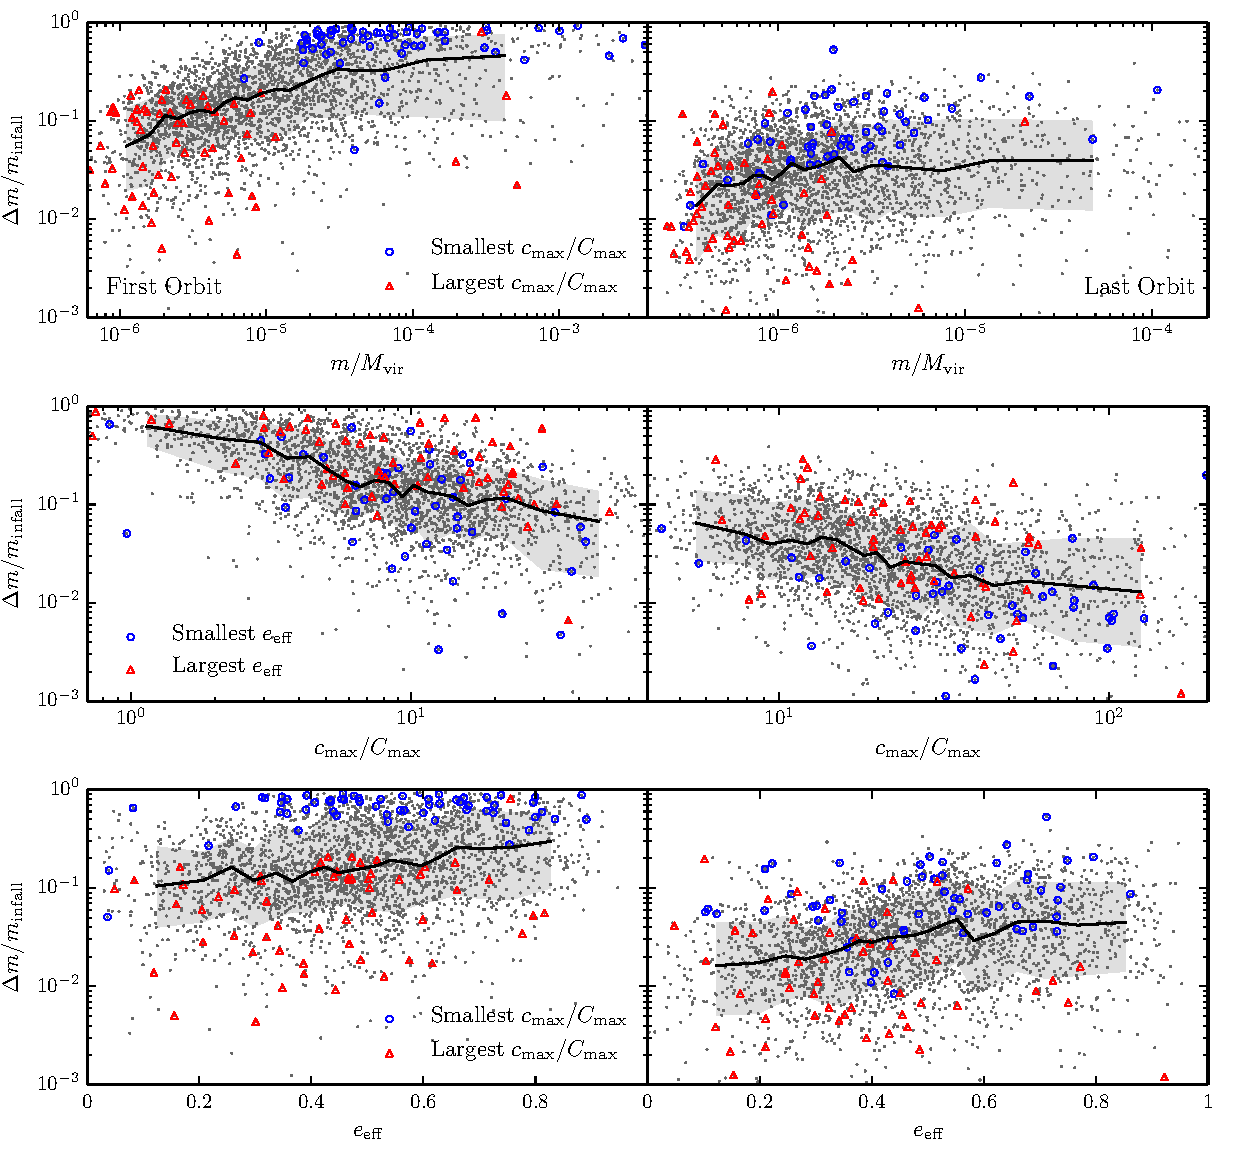
\includegraphics[width=\smwidth]{./figures/neutrinos/fig11.pdf} \vspace{-0.1cm}
\caption[Correlation length as a function of neutrino mass]
{The correlation length defined to be the distance for
which the correlation function in equation (\ref{eq:corrfun}) drops
to half its maximum value for varying neutrino masses.  The
simulations have longer correlation lengths but follow a
similar power law behaviour.}
\vspace{-0.2cm}
\label{fig:corrlength}
\end{center}
\end{figure}
% -------------------------------------------- FIGURE 11 --------------------------------------------

% ================================================================================
% DISCUSSION
% ================================================================================  
  
\section{Discussion}
\label{sec:discussion}
  
We have tested four methods of computing the velocity field: a nearest particle method, a momentum method, and reconstruction via CDM and halo density fields.  Our results are generally consistent with theoretical expectations and highly correlated among each other.  Specifically we have demonstrated that reconstructing the velocity from point-particle halos produces a velocity field highly correlated with that of our $N$-body particles.  It is the near unit correlation coefficient - a measure of the angle between the two fields - that ensures that the reconstructed velocity points in the right direction.  The magnitude of the velocity can then simply be scaled to the correct value as long as the bias is known. 

This result allows for a prescription to determine the actual velocity fields in our own Universe.
\begin{enumerate}
\item Reconstruct the galaxy density field from a galaxy survey catalogue. We expect this reconstruction to be very comparable to the halo reconstruction we use here except with the addition of a 1-halo term to make the bias constant over more wavenumbers.
\item Fourier transform the gridded density field.  Then, use equation (\ref{eq:vrec}) to compute the CDM, neutrino and relative velocity fields in Fourier space.  Here, a nonlinear correction can be applied by additionally multiplying by a factor of $\Delta_v^{\rm Sim}/\Delta_v^{\rm Rec HA}$.
\item Fourier transform back to real space.
\end{enumerate}
We first note that a similar process could be performed on the density fields produced by 21 cm observations.  We also note that redshift distortions and masking effects might result in extra biases in the reconstruction scheme.  We intend to investigate these effects in a future paper. 
  
Our results also provide support for the applicability of the analysis performed in \citet{zhu/etal:2014b,zhu/etal:2014a}.  They used moving background perturbation theory to study the neutrino relative velocity effect.  The moving background approximation relies on having a coherent background relative flow and our simulation results indicate that the coherency scales of such motions are larger than predicted.  Thus, we expect that inaccuracies in the predicted dipole distortion to the correlation function will come from nonlinear evolution rather than the moving background approximation.  We note that we can also directly measure the dipole correlation function in our simulations and plan to report on this in a subsequent paper.  
  
% ================================================================================
% CONCLUSION
% ================================================================================  
  
\section{Conclusion}
\label{sec:conclusion}
  
We performed a set of four large $N$-body simulations including cold dark matter and neutrinos of varying mass.  We have accurately measured the cold dark matter-neutrino relative velocity.  We find that we can accurately reconstruct this velocity using a linear theory approach and halo density fields.  We have described a simple method for accurately predicting the relative velocity field via a galaxy survey or 21 cm observations.  Since such a reconstruction allows for an independent measurement of neutrino masses, we expect this technique to provide significant constraints in upcoming astronomical surveys.  

% ================================================================================
% ACKNOWLEDGEMENTS
% ================================================================================

\section*{\centering Acknowledgements}

We acknowledge valuable discussions with Joel Meyers, Yu Yu and Francisco Villaescusa-Navarro.  We acknowledge the support of NSERC. Computations were performed on the GPC supercomputer at the SciNet HPC Consortium \citep{loken/etal:2010}. SciNet is funded by: the Canada Foundation for Innovation under the auspices of Compute Canada; the Government of Ontario; Ontario Research Fund - Research Excellence; and the University of Toronto.
  

%\include{./sections/frb_modelling}
%\include{./sections/frb_statistics}
%\include{./sections/tiannu}
%\include{./sections/conclusions}

% ==============================================================================
% BIBLIOGRAPHY
% ==============================================================================

\addcontentsline{toc}{chapter}{Bibliography} % Adds a line for the Bibliography in the Table of Contents.

\bibliographystyle{apj}
\bibliography{references}

\end{document}
